\chapter{Resultate}\label{chap:r} 

Die Resultate tragen die in der Testumgebung erfassten Daten und Werte über die
KI zusammen. Für die verschiedenen Variationen und Kriterien werden nachfolgend
Abkürzungen eingeführt, die für die Präsentation und die Diskussion der
Resultate fortan verwendet werden.

Die Abkürzungen der Kriterien lauten:
\begin{itemize}
    \item Sim (siehe \doubleref{sub:m_eval_proc})
    \item Rec (siehe \doubleref{sub:m_eval_rec})
    \item Speed (siehe \doubleref{sub:m_eval_speed})
    \item Drawtime  (siehe \doubleref{sub:m_eval_zeichnend})
    \item Overdrawn (siehe \doubleref{sub:m_eval_uebermalung})
\end{itemize}

Die Abkürzungen der Variationen der nachzeichnenden KI lauten: 
\begin{itemize}
    \item Base (siehe \doubleref{sub:m_var_base})
    \item Rec (siehe \doubleref{sub:m_var_rec})
    \item Speed (siehe \doubleref{sub:m_var_speed})
    \item No-Penlift (+ Speed) (siehe \doubleref{sub:m_var_penlift})
    \item No-Overdraw (siehe \doubleref{sub:m_var_overdraw})
    \item Physics (siehe \doubleref{sub:m_var_phy})
\end{itemize}

Die Abkürzungen der Variationen der generativen KI lauten:
\begin{itemize}
    \item Deterministic
    \item Softmax
\end{itemize}





\section{Tabellen}\label{chap:r_tab} 

Der erste Teil der Resultate besteht aus Tabellen, welche die Daten über die
Leistung der KI aus der Testumgebung (siehe \doubleref{chap:m_auswert}) zusammentragen. Die Tabellen sind dabei in
diejenigen der nachzeichnenden KI und diejenigen der generativen KI unterteilt.

\subsection{Tabellen der nachzeichnenden KI}\label{sub:r_tab_nachzeich}
Die Tabellen für die nachzeichnende KI beschreiben die Leistung jeder Variation
in jedem Kriterium. Es gibt insgesamt drei Tabellen für die nachzeichnende KI.
Der Unterschied in den Tabellen liegt im Datenset, mit denen die KI jeweils
getestet wurde.

\begin{table}[!ht]
    \centering
    \caption{Testen auf MNIST Datenset | 2000 Tests}\label{tab:MNIST}
    \begin{tabular}{|l|l|l|l|}
        \hline
            ~ & Übereinstimmung \% & Erkennbarkeit \% & Geschwindigkeit \\ \hline
            Grund-Basis & 86.5 & 86.6 & 24.5 \\ \hline
            Grund-MNIST & 66.8 & 64.3 & 51.2 \\ \hline
            Grund-Speed & 85.7 & 82.3 & 23.3 \\ \hline
            Grund-MNIST-Speed & 61.4 & 55.1 & 56.8 \\ \hline
            Physik-Basis & 56.4 & 46.4 & 62.5 \\ \hline
            Physik-MNIST & 38.4 & 35.7 & 63.9 \\ \hline
            Physik-Speed & 63.0 & 58.2 & 61.2 \\ \hline
            Physik-MNIST-Speed & 29.2 & 27.3 & 63.7 \\ \hline
        \end{tabular}
\end{table}

\begin{table}[!ht]
    \centering
    \caption{Testen auf EMNIST Letters Datenset | 2000 Tests}\label{tab:EMNIST}
    \begin{tabular}{|l|l|l|l|}
    \hline
        ~ & Übereinstimmung \% & Erkennbarkeit \% & Geschwindigkeit \\ \hline
        Grund-Basis & 86.8 & 74.5 & 38.2 \\ \hline
        Grund-MNIST & 65.2 & 45.0 & 57.4 \\ \hline
        Grund-Speed & 88.1 & 73.5 & 36.1 \\ \hline
        Grund-MNIST-Speed & 62.2 & 40.0 & 60.9 \\ \hline
        Physik-Basis & 57.6 & 32.4 & 63.5 \\ \hline
        Physik-MNIST & 43.3 & 23.6 & 63.9 \\ \hline
        Physik-Speed & 56.3 & 35.0 & 63.6 \\ \hline
        Physik-MNIST-Speed & 30.2 & 13.9 & 64.0 \\ \hline
    \end{tabular}
\end{table}

\begin{table}[!ht]
    \centering
    \caption{Testen auf QuickDraw-Datenset | 2000 Tests}\label{tab:Quickdraw}
    \begin{tabular}{|l|l|l|l|}
    \hline
        ~ & Übereinstimmung \% & Erkennbarkeit \% & Geschwindigkeit \\ \hline
        Grund-Basis & 79.1 & 80.5 & 39.1 \\ \hline
        Grund-MNIST & 57.3 & 62.5 & 59.9 \\ \hline
        Grund-Speed & 80.0 & 80.3 & 35.0 \\ \hline
        Grund-MNIST-Speed & 54.9 & 58.9 & 62.5 \\ \hline
        Physik-Basis & 48.1 & 55.7 & 63.8 \\ \hline
        Physik-MNIST & 30.5 & 38.9 & 64.0 \\ \hline
        Physik-Speed & 50.0 & 58.3 & 63.6 \\ \hline
        Physik-MNIST-Speed & 22.4 & 31.1 & 64.0 \\ \hline
    \end{tabular}
\end{table}


\subsection{Tabellen der generativen KI}\label{sub:r_tab_gen}
Die Tabellen der generativen KI beschreiben die Leistung der zugehörigen
Variationen auf die ausgewählten Kriterien. Es gibt insgesamt fünf Tabellen.
Jede Tabelle beschreibt die Leistung im Zeichnen eines des ausgewählten Motive.


\begin{table}[!ht]
    \centering
    \caption{Testen auf QuickDraw-Datenset | 2000 Tests}\label{tab:Quickdraw}
    \begin{tabular}{|l|l|l|l|}
    \hline
        ~ & Übereinstimmung \% & Erkennbarkeit \% & Geschwindigkeit \\ \hline
        Grund-Basis & 79.1 & 80.5 & 39.1 \\ \hline
        Grund-MNIST & 57.3 & 62.5 & 59.9 \\ \hline
        Grund-Speed & 80.0 & 80.3 & 35.0 \\ \hline
        Grund-MNIST-Speed & 54.9 & 58.9 & 62.5 \\ \hline
        Physik-Basis & 48.1 & 55.7 & 63.8 \\ \hline
        Physik-MNIST & 30.5 & 38.9 & 64.0 \\ \hline
        Physik-Speed & 50.0 & 58.3 & 63.6 \\ \hline
        Physik-MNIST-Speed & 22.4 & 31.1 & 64.0 \\ \hline
    \end{tabular}
\end{table}




\section{Bildersammlung}\label{chap:r_bild} Eine Sammlung von gezeichneten
Strichbildern ergänzt die Resultate. Die Zeichnungen, die in der Sammlung
vertreten sind, stammen aus einer zufälligen Auswahl aus dem Test der jeweiligen
Variation der KI. Die Bilder haben einen Farbverlauf, der den zeitliche Verlauf
des Zeichnens darstellt. Die Helligkeit eines Striches ist proportional zu dem
Step, in dem dieser gezeichnet wurde. Das bedeutet, dass dunklere Striche früher
gezeichnet wurden als hellere Striche. Bewegungen des Agents, in denen dieser
nicht zeichnete, sind in den Bildern nicht erkennbar.


\subsection{Bildersammlung der nachzeichnenden KI}\label{sub:r_bild_nach}

Die Strichbilder für die Bildersammlung der nachzeichnenden KI sind jeweils in Paaren
angeordnet. Das linke Bild im Paar zeigt die Vorlage aus dem Datenset und das
rechte Bild zeigt die nachgezeichnete Variante von der KI. Jede Spalte der
Bildersammlung zeigt Bilder aus einem anderen Datenset

\begin{figure}[!ht]
    \centering
    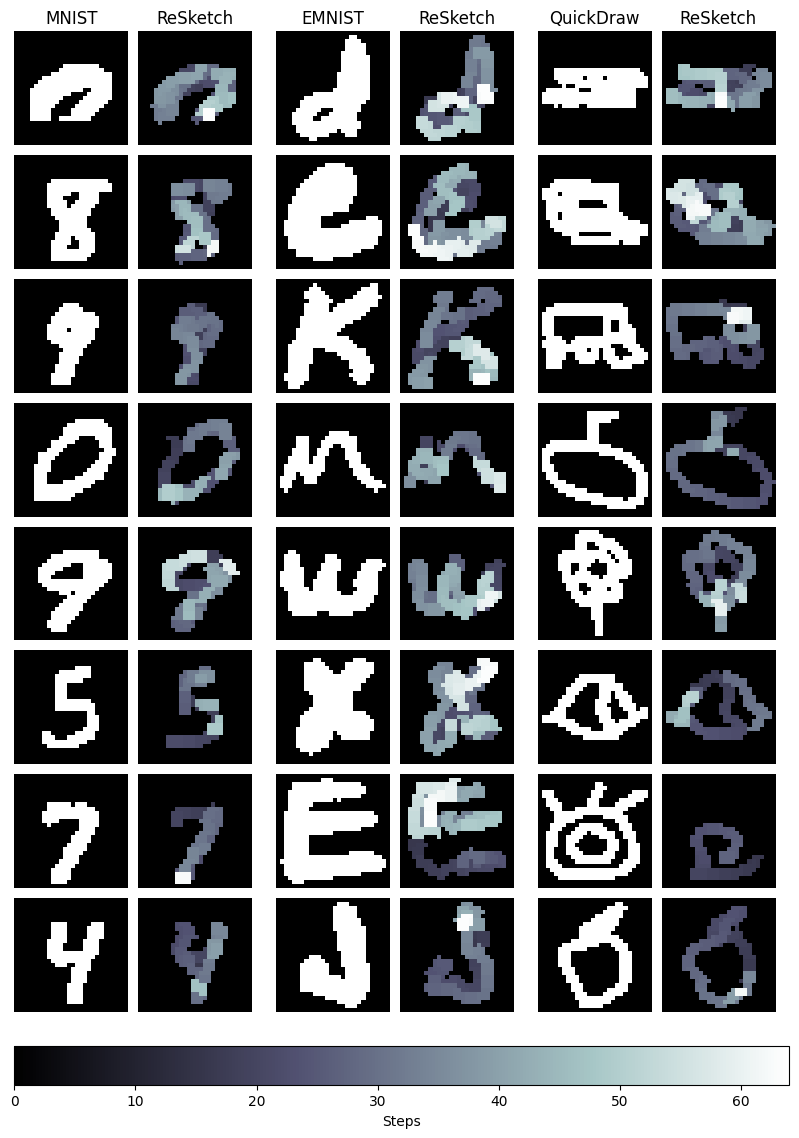
\includegraphics[width=\textwidth]{images/resultate/base-base.png}
    \caption{Grund-Basis Bildersammlung}\label{fig:Grund-Basis}
\end{figure}

\newpage
\begin{figure}[!ht]
    \centering
    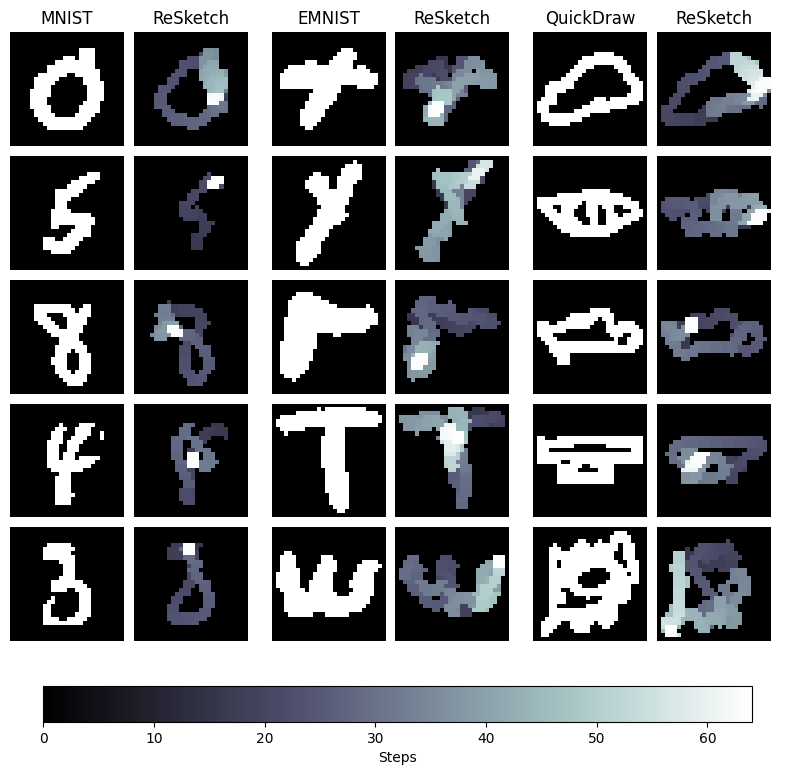
\includegraphics[width=\textwidth]{images/resultate/base-mnist.png}
    \caption{Grund-MNIST Bildersammlung}
    \label{fig:Grund-MNIST}
\end{figure}

% \begin{figure}[!ht]
%     \centering
%     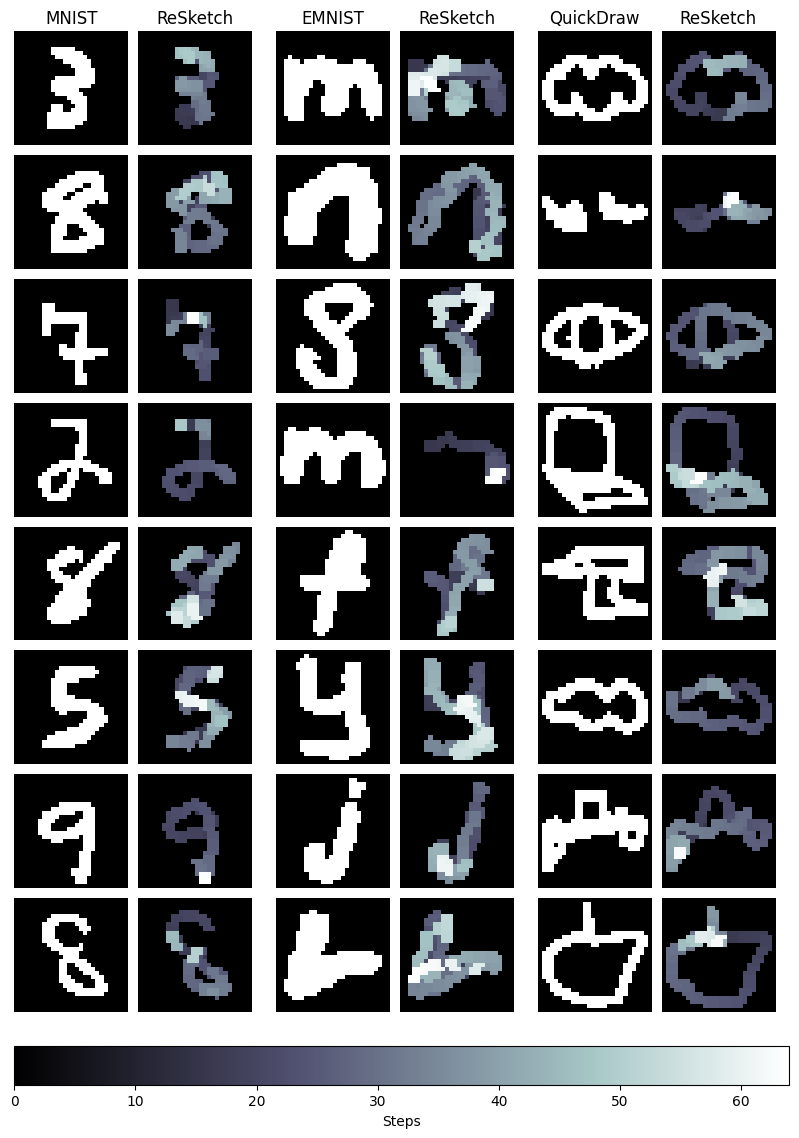
\includegraphics[width=\textwidth]{images/resultate/base-speed.png}
%     \caption{Grund-Speed}
%     \label{fig:Grund-Speed}
% \end{figure}

\begin{figure}[!ht]
    \centering
    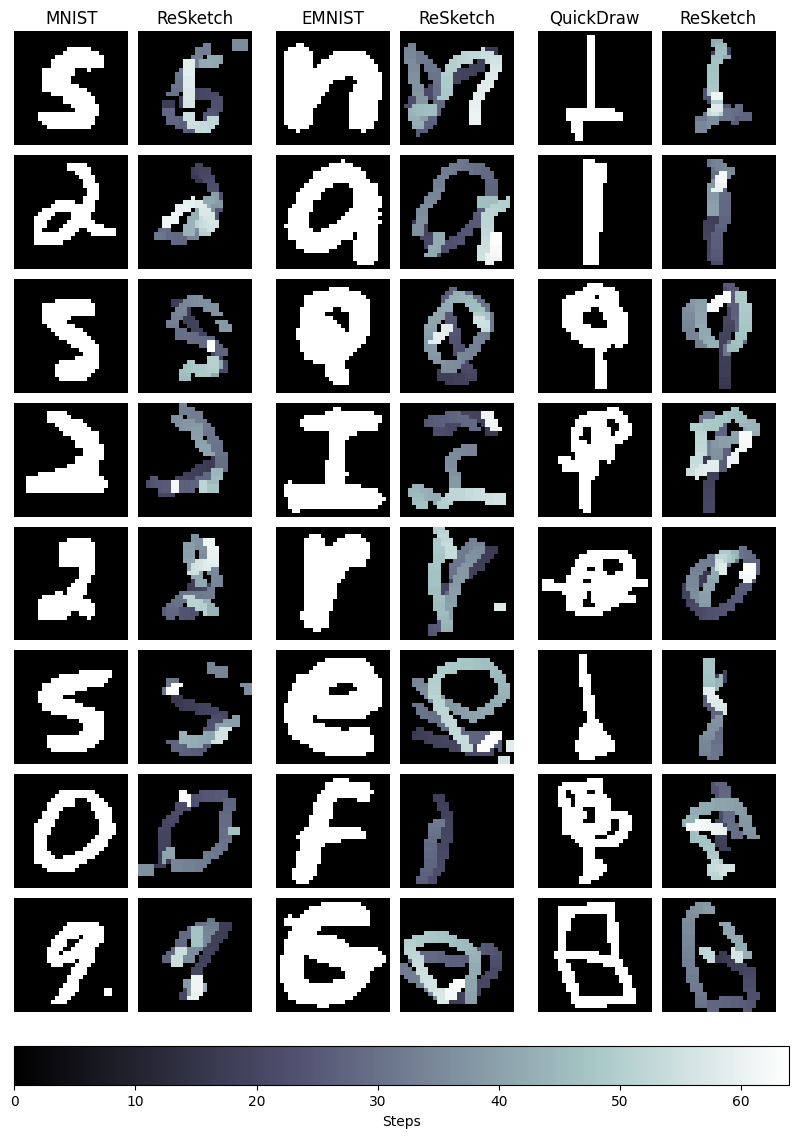
\includegraphics[width=\textwidth]{images/resultate/physics-base.png}
    \caption{Physik-Basis Bildersammlung}\label{fig:Physik-Basis}
\end{figure}

\begin{figure}[!ht]
    \centering
    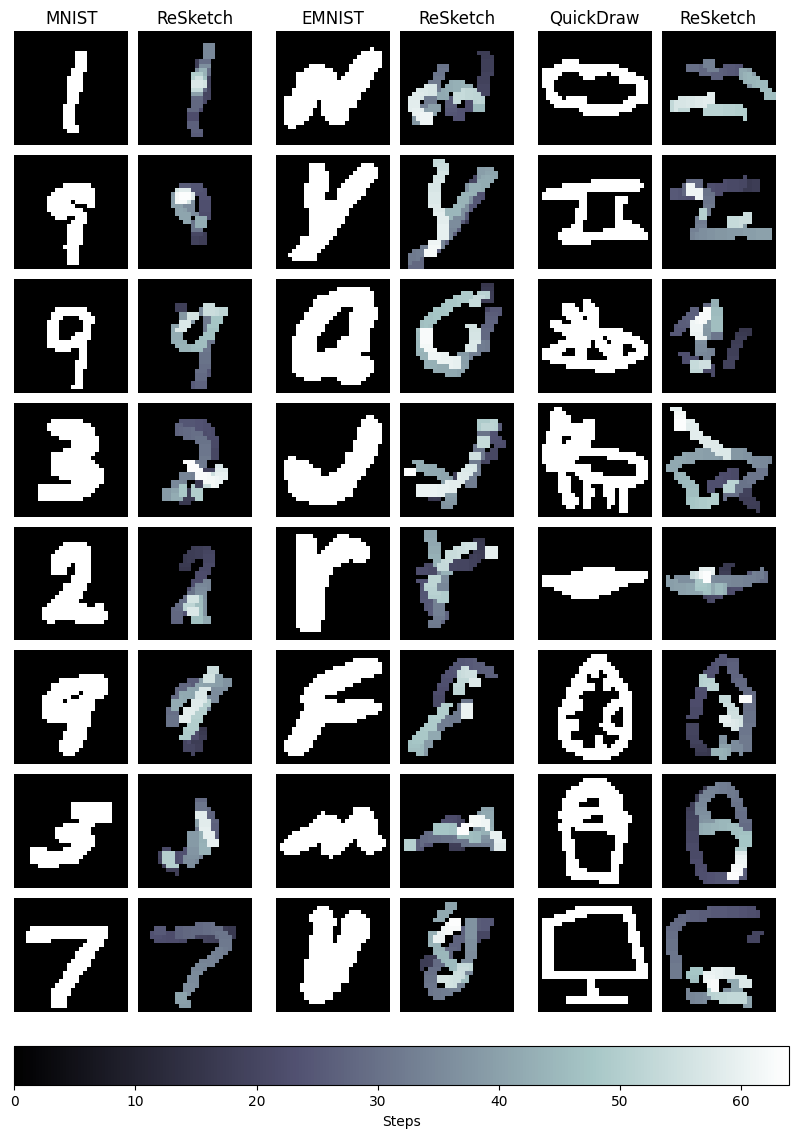
\includegraphics[width=\textwidth]{images/resultate/physics-speed.png}
    \caption{Physik-Speed Bildersammlung}
    \label{fig:Physik-Speed}
\end{figure}


\subsection{Bildersammlung der nachzeichnenden KI}\label{sub:r_bild_nach}

Die Bildersammlung für eine Variation der generativen KI hat fünf Spalten. Jede
Spalte zeigt Zeichnungen der KI von einem der ausgewählten Motive (siehe
\doubleref{sub:m_auswert_gen}).
